\documentclass[twocolumn, 9pt]{article}

\usepackage[toc,page]{appendix}
\usepackage[T1]{fontenc}
\usepackage{algpseudocode}
\usepackage{amsmath}
\usepackage{amssymb}
\usepackage{balance}
\usepackage{booktabs} % For formal tables
\usepackage{caption}
\usepackage{enumitem}
\usepackage{hyperref}
\usepackage{listings}
\usepackage{multirow}
\usepackage{subcaption}
\usepackage{tikz}
\usepackage{usenix}
\usepackage{varwidth}
\usepackage{xcolor}

\usepackage[explicit]{titlesec}

\hypersetup{
  colorlinks=true,
  linkcolor=ACMRed,
  urlcolor=ACMBlue,
  citecolor=ACMRed,
}

\definecolor[named]{ACMBlue}{cmyk}{1,0.1,0,0.1}
\definecolor[named]{ACMYellow}{cmyk}{0,0.16,1,0}
\definecolor[named]{ACMOrange}{cmyk}{0,0.42,1,0.01}
\definecolor[named]{ACMRed}{cmyk}{0,0.90,0.86,0}
\definecolor[named]{ACMLightBlue}{cmyk}{0.49,0.01,0,0}
\definecolor[named]{ACMGreen}{cmyk}{0.20,0,1,0.19}
\definecolor[named]{ACMPurple}{cmyk}{0.55,1,0,0.15}
\definecolor[named]{ACMDarkBlue}{cmyk}{1,0.58,0,0.21}

\lstset{
  captionpos=b,
  showspaces=false,
  showtabs=false,
  breaklines=true,
  showstringspaces=false,
  breakatwhitespace=true,
  escapeinside={(*@}{@*)},
  basicstyle=\footnotesize\ttfamily,
  columns=fullflexible,
  morekeywords={maybe_downsample, maybe_skip, maybe}
}

\captionsetup[lstlisting]{font={footnotesize}}
\renewcommand{\lstlistingname}{Example}

\makeatletter
\newcommand\appendix@section[1]{%
  \refstepcounter{section}%
  \orig@section*{Appendix \@Alph\c@section: #1}%
  \addcontentsline{toc}{section}{Appendix \@Alph\c@section: #1}%
}
\let\orig@section\section
\g@addto@macro\appendix{\let\section\appendix@section}
\makeatother

\newcommand*{\Appendixautorefname}{Appendix}

\frenchspacing

\begin{document}

% don't want date printed
\date{}

\newcommand{\sysname}{AdaptiveStream}
\newcommand{\para}[1]{\smallskip\noindent\textbf{#1}}
\newcommand{\paraf}[1]{\smallskip\noindent\textbf{#1}}
\newcommand{\todo}[1]{{\color{ACMRed}\bf{TODO: #1}\normalfont}}

\def\Snospace~{\S{}}
\renewcommand*\sectionautorefname{\Snospace}
\renewcommand*\subsectionautorefname{\Snospace}
\renewcommand*\subsubsectionautorefname{\Snospace}
\renewcommand*{\equationautorefname}{Eq.}
\renewcommand*{\figureautorefname}{Fig.}

%%% Local Variables:
%%% mode: latex
%%% TeX-master: "sosp17"
%%% End:


\title{\sysname{}: Adaptive Wide-Area Streaming Analytics}

\author{
  \textit{Anonymous for submission}
}

\maketitle

\subsection*{Abstract}

The emerging class of wide-area streaming analytics faces the challenge of
scarce and variable WAN bandwidth. Applications that solely rely on transport
protocols like TCP and UDP suffer from increased latency or degraded
accuracy. Existing approaches that adapt to network changes are often
application-specific or require extensive developer effort.

We present \sysname{}, a stream processing system that simultaneously achieves
low latency and high accuracy in the wide area, requiring minimal developer
effort. To realize this, \sysname{} uses three ideas: $(i)$ it integrates
application adaptation as a first-class programming abstraction in the stream
processing model; $(ii)$ with a combination of offline and online profiling, it
automatically learns an accurate and precise profile that models accuracy and
bandwidth trade-off; and $(iii)$ at runtime, it adjusts the application data
rate to match the available bandwidth. We evaluate \sysname{} using three
real-world applications: pedestrian detection, augmented reality, and monitoring
log analysis. Our experiments show that \sysname{} achieves sub-second latency
with nominal accuracy drop.

\section{Introduction}

%% Background
Wide-area streaming analytics are becoming pervasive, especially with the
emerging class of Internet of Things (IoT) applications.  Large cities such as
London and Beijing have deployed millions of cameras for surveillance and
traffic control~\cite{skynet, london.surveillance}. Buildings are increasingly
equipped with a wide variety of sensors to improve energy efficiency and
occupant comfort~\cite{krioukov2012building}. Geo-distributed infrastructure,
such as content delivery networks (CDNs), analyzes requests from machine logs
over the globe~\cite{mukerjee2015practical}. These applications need to
transport, distill and process streams of data across the wide area in real
time.

Although existing stream processing systems, such as
Storm~\cite{toshniwal2014storm}, Spark Streaming~\cite{zaharia2013discretized},
and VideoStorm~\cite{zhang2017live}, can handle large streams of data, they are
designed to work within a single cluster, where the network is not the
bottleneck.  In contrast, the wide area network (WAN) has limited
bandwidth~\cite{hsieh17gaia, vulimiri2015global}. Moreover, WAN bandwidth growth
has been decelerating for many years~\cite{global2016telegeography} while
traffic demands are growing at a staggering rate~\cite{index2013zettabyte}.

Limited WAN bandwidth makes it neither practical nor efficient to back-haul all
data to a central location.  Recent research on WAN-aware systems promotes
pushing computations towards the edge~\cite{pu2015low, rabkin2014aggregation,
  satyanarayanan2009case}. However, communication is not entirely avoidable:
$(i)$ some analytical jobs require joining or aggregating data from multiple
geo-distributed sites~\cite{pu2015low, viswanathan2016clarinet}; $(ii)$ the edge
benefits substantially from central computing resources such as GPUs and
TPUs~\cite{abadi2016tensorflow} in the cloud; and $(iii)$ end-devices such as
cameras and mobile devices suffer from limited bandwidth in last-hop wireless
links when running processing on nearby edge
infrastructure~\cite{abari2017enabling, zhang2015design}.

% could improve efficiency (such as GDA pushes queries out; cloudlet
% etc). However, we still need data transmission for cloud off-loading or
% aggregation purpose.

When facing insufficient bandwidth, application developers need to make a
decision within the design space of data fidelity versus freshness
(\autoref{fig:intro}).

\begin{figure}
  \centering
  \includegraphics[width=0.8\columnwidth]{figures/figure1.pdf}
  \caption{The trade-off space between data freshness and fidelity when facing
    insufficient bandwidth (details in \autoref{sec:runtime-adaptation}).}
  \label{fig:intro}
  \vspace{-1em}
\end{figure}

Applications using existing protocols without adaptation result in extreme
design points. Streaming over TCP ensures a reliable delivery but backlogged
data increases latency. On the other hand, streaming over UDP minimizes latency
by sending packets as fast as possible, but uncontrolled loss devastates
application accuracy.

Degradation, as demonstrated by JetStream~\cite{rabkin2014aggregation}, allows
developers to trade data fidelity for freshness. While it's easy to write
policies for simple operations, such as sampling, in general, accurate policies
will require extensive expertise and considerable efforts. In practice,
developers write policies based on some set of heuristics rather than
quantitative measurements. These inaccurate manual degradation policies lead to
sub-optimal performance for both freshness and fidelity.

Furthermore, application-specific optimizations do not generalize. A fine-tuned
adaptation algorithm for one application will work poorly for another
application, if performance metrics or data distributions change.  For example,
video streaming focuses on quality of experience
(QoE)~\cite{michalos2012dynamic, pantos2016http, yin2015control}. Because humans
favor smoothness over image quality, video streaming systems maintain a high
frame rate, e.g.\,\(25~\text{FPS}\), and reduce image resolutions under
bandwidth limit.  Adaptation by reducing resolutions is a poor match for
analytic jobs that rely on image details.

To achieve low latency and high accuracy simultaneously with minimal developer
effort, we design and implement \sysname{}, a stream processing system for the
wide area. The key idea is to build an accurate and precise performance model
instead of relying on manual or application-specific policies. \sysname{}'s
solution is three-fold: easy-to-use APIs, automatic profiling, and a low-latency
runtime.

\sysname{} augments existing stream processing operators with a new \maybe{}
operator. Its basic form takes a list of values as a knob and a function that
degrades the input stream. The knob specifies the degradation level that affects
data size and data fidelity. We extend the basic form with a library of
specialized operators for common data types, such as \texttt{maybe\_downsample}
for images. Our APIs are simple, composable and extensible. Developers do not
need to be an expert in the application domain as the knobs tolerate approximate
specifications. Multiple operators form a configuration that affects the
adaptation jointly. Arbitrary functions and external libraries can be embedded
with our operators.

\sysname{} then uses a data-driven approach to automatically build application
performance profiles with minimal developer effort. The profiles accurately
capture the relationship between application accuracy and bandwidth consumption
under different combinations of data degradation operations. We use an offline
process to bootstrap our system with developer-supplied training data, and
continuously refine the profile online to handle model drifts. We exploit
parallelism and sampling-based profiling to efficiently explore the
configuration space and learn a Pareto-optimal adaptation strategy.

At runtime, \sysname{} achieves low latency by matching data rate to available
bandwidth, and high accuracy by using Pareto-optimal configurations from the
profile. Upon network congestion, our rate adaptation algorithm increases the
degradation level to reduce data rate, such that no persistent queue builds
up. To recover, it progressively decreases the degradation level after probing
for more available bandwidth. The runtime also provides additional options for
developers to control application behaviors, e.g., limiting the maximum allowed
WAN bandwidth. For multiple applications, the profiles allow bandwidth
allocation among competing tasks for utility fairness.

To evaluate \sysname{}, we've built three streaming applications: augmented
reality (AR), pedestrian detection (PD), and distributed Top-K analysis (TK). We
use real-world data to profile these applications and evaluate their runtime
performance on a geo-distributed public cloud. Our contributions and evaluation
results are as follows.

\begin{itemize}[leftmargin=*, topsep=2pt, itemsep=2pt]

\item We propose \maybe{} operators to incorporate adaptation with existing
  stream processing models. Our programming abstraction is simple, composable
  and extensible.

\item We show that \sysname{}'s data-driven approach generates an accurate and
  precise profile for each application. Parallelism and sampling techniques
  can speed up the profiling substantially, up to 29$\times$ and 9$\times$\@.

\item Using runtime experiments on geo-distributed EC2 nodes, \sysname{}
  achieves low latency and high accuracy simultaneously for all
  applications---sub-second latency and 2\% accuracy drop for video analytics,
  4-second latency and 1\% accuracy drop for TK\@.

\end{itemize}

%%% Local Variables:
%%% mode: latex
%%% TeX-master: "awstream"
%%% End:

%% LocalWords: VideoStorm, analytics, CDN, IoT

\section{Motivation}
\label{sec:background-motivation}

In this section, we make the case for an adaptive stream processing system in
the wide area by examining the gap between application demands and the existing
infrastructure. We start with a few streaming applications.

\para{Video Surveillance:} We envisage a city-wide monitoring system that
aggregates camera feeds (both stationary ground cameras and moving aerial
vehicles) and analyzes video streams in real-time for surveillance, anomaly
detection or business intelligence~\cite{oh2011large}. While traditionally human
labors are involved in analyzing abnormal activities, recent advances in
computer vision and deep learning has dramatically increased the accuracy for
automatic analysis of visual scenes, such as pedestrian
detection~\cite{dollar2012pedestrian}, vehicle tracking~\cite{coifman1998real},
or facial recognition to locate people of interest~\cite{parkhi2015deep,
  Lu:2015:SHF:2888116.2888245}. \todo{Add concrete numbers to argue for the data
  volume.}

\para{IoT Sensors:} While traditional environmental sensors are
slow~\cite{atzori2010internet}, we are seeing an increasing trend with
high-frequency, high-precision sensors being deployed. For example, uPMU
monitoring system for the electrical grid consists of a network of 1000 devices;
each produces 12 streams of 120 Hz high-precision values accurate to 100
ns. This amounts to 1.4 million points per second that requires specialized
timeseries database~\cite{andersen2016btrdb}.

\para{Log Analysis:} Large organizations today are managing 10--100s of
datacenters (DCs) and edge clusters worldwide~\cite{calder2013mapping}. While
most log analysis today runs in a batch mode and on a daily basis, there is
trend in analyzing logs in real-time for quicker optimization \todo{cite RISE
  reference?}. For example, a content distribution network (CDN) can improve the
overall efficiency by optimizing data placement if the access logs can be
processed in real-time.

\vspace{0.5em}

We consider the practical issues with deploying these applications. While they
challenge the data storage and processing system, the cloud can handle it well.
The real challenge lies in the communication. Data generated from the edge, not
a lot WAN bandwidth; also with cost. And worse, the bandwidth is also not
guaranteed. We will demonstrate with measurement.

\subsection{Wide-Area Bandwidth Characteristics}
\label{sec:making-case-adapt}

\begin{figure}
  \centering
  \includegraphics[width=.95\linewidth]{figures/europe-to-us-west.pdf}
  \caption{Bandwidth measurement between Amazon EC2 sites (from Ireland to
    California).}
  \label{fig:bw}
\end{figure}

To understand the bandwidth characteristics in the wide-area, we conducted a
simple measurement using Amazon EC2. We use iPerf~\cite{iperf} to measure the
pair-wise bandwidth between four geo-distributed sites throughout the day. We
observed large variance in the measured bandwidth and one such pair is shown in
\autoref{fig:bw}. Regardless of the number of flows\footnote{EC2 has a per-flow
  and per-VM rate limiting~\cite{zhang2016guaranteeing}.}, these exist occasions
when the available bandwidth is almost halved. We believe the backhaul links
between EC2 sites are better (if not at least representative) in comparison to
the general wide-area links. The varying nature poses real challegen to the
realization and successful deployment of wide-area streaming applications.

\subsection{Bandwidth-Accuracy Trade-off}
\label{sec:bat}

% Existing stream processing systems in the wide area often directly use TCP as
% their transport. TCP works remarkably well estimating the available bandwidth
% and minizing flow completion time. Although TCP adapts the congestion window in
% dynamically based on the feedback from the
% receiver~\cite{jacobson1988congestion}, being application agnostic, TCP delivers
% whatever the application wants to send; and in the case of limited network
% capacity, TCP creates backlogged data, causing significant delay.

% For applications where TCP's retransmission is not unnessary, UDP is often
% chosen. Many multimedia applications such as Internet
% telephony~\cite{baset2004analysis}. Live IP cameras streaming with RTMP. Or
% sensor data over OSC~\cite{wright1997open}, a protocol based on UDP. UDP's
% packet loss can be detrimental in the deteriorate situations.

% The issue with these protocol is that they are designed to be generally
% applicable to many applications without intervening the application execution.
% Often developers of individual applications need to tune the transport to fit
% their needs~\cite{tierney2001tcp} or deal with the insufficient bandwidth case.

The edge infrastructure is capable of pre-processing the data before the
communication. Data degradation. Such as frame-diff based video encoding
scheme. In the case of the top-K application, we first generate windowed local
counts. In our dataset, we see 100x data size reduction. While effective, these
transformations are often not sufficient. In the case of top-k, there is a long
tail. In the case of images/video, quantizing individual pixels will often give
more space.

They help reduce the resource demand but they typically also lower the output
quality. \autoref{fig:log-trade-off} shows how the image resolution affects
application accuracy.

In some verticle domain, such as video encoding, adaptive scheme
exists. However, there is no general solution and these solutions are not
generally applicable to all applications. Most video encoding techniques will
adjust the quantizer to tune the encoding size and quality; while often
preserving the frame rate as these videos are for human consumption. A smooth
video provides a better quality of experience than higher resolution but
intermitten images.

We presented empirical results with grouped, windowed aggregation on PlanetLab
using Akamai log data, and highlighted the complexity of tradeoffs that we show
are driven by several factors such as query, data, and resource
characteristics. local aggregation and global
aggregation.~\cite{heintz2015towards}

This motivates us to design an application-aware rate-adapting stream processing
framework for the wide area; primarily exploring the design space of
degradation.

For these applications, there is a trade-off between the bandwidth and accuracy.
Exploring the design space that allows explicit trading accuracy for resource
constrained cases is the main goal of this paper.

\begin{figure}
  \centering
  \begin{subfigure}{.48\columnwidth}
    \centering
    \includegraphics[width=.95\linewidth]{figures/motiv-resolution.pdf}
    \label{fig:log-bw}
  \end{subfigure}
  \begin{subfigure}{.48\columnwidth}
    \centering
    \includegraphics[width=.95\linewidth]{figures/motiv-framerate.pdf}
    \label{fig:log-acc}
  \end{subfigure}
  \caption{The trade-off between required bandwidth and the accuracy.}
  \label{fig:log-trade-off}
\end{figure}

%%% Local Variables:
%%% mode: latex
%%% TeX-master: "sigcomm2017"
%%% End:

\section{\sysname{}}
\label{sec:system}

In contrast to existing approaches that require developers to specify the
concrete policies, \sysname{} uses a special operator \texttt{maybe} to express
structured adaptation. The specifications are hints on potential operations
without exact quantifications. \sysname{} then automatically learns concrete
degradation strategies (the profile) using profiling data (either offline or
online) and controls the application execution at runtime. The profiles also
have additional benefits such as coordination among competing streaming
flows. \autoref{fig:overview} provides an overview of the systems (in three
stages) and we describe each stage in turn.

\begin{figure}
  \centering
  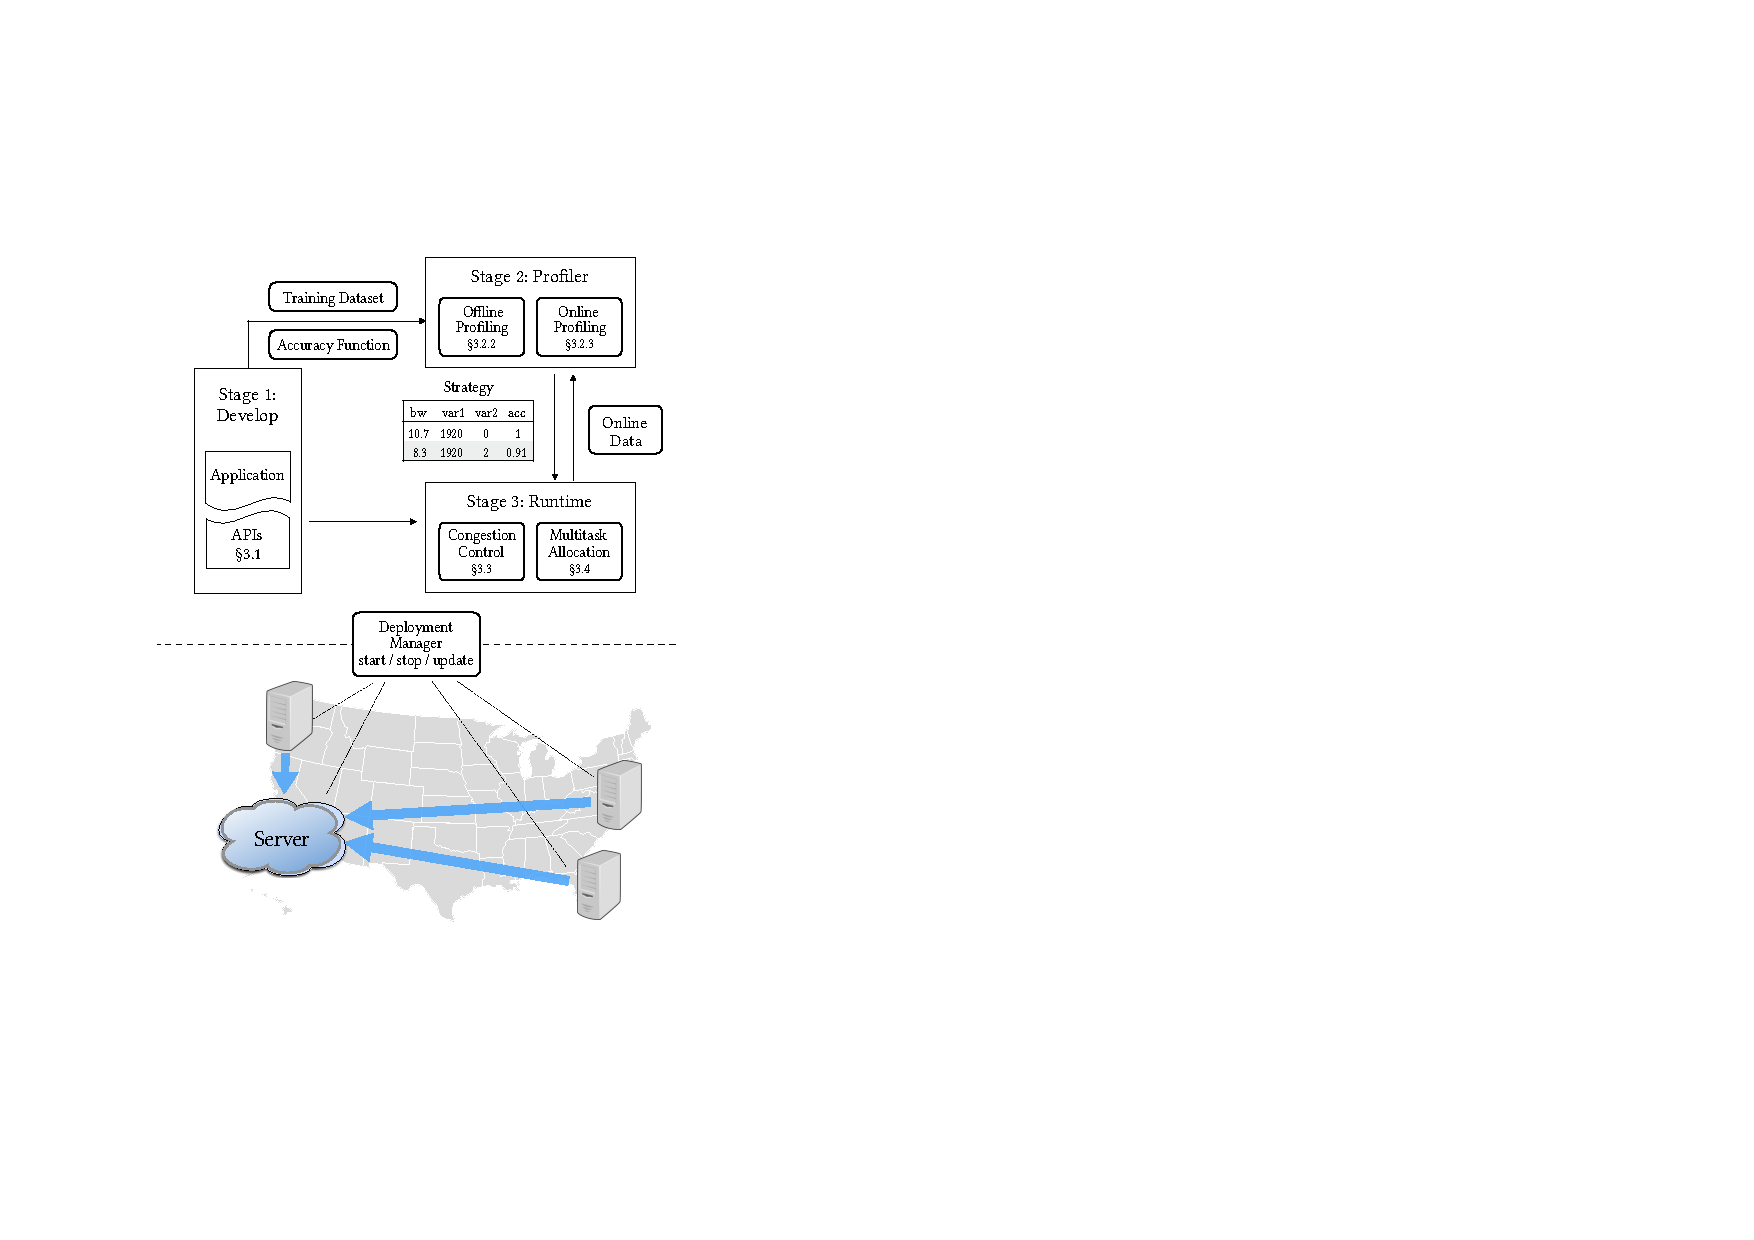
\includegraphics[width=.9\linewidth]{figures/system.pdf}
  \caption{High-level overview of \sysname{}.}
  \label{fig:overview}
\end{figure}

\begin{table*}
  \small
  \centering
  \begin{tabular}{ c r l }
    \toprule
    \multirow{5}{*}{Normal Operators}
    & \textit{map} (f: I $\Rightarrow$ O) & Stream<I> $\Rightarrow$ Stream<O> \\
    & \textit{skip} (i: Integer) & Stream<I> $\Rightarrow$
                                   Stream<I> \\
    & \textit{sliding\_window} (count: Integer, f: Vec<I> $\Rightarrow$ O) & Stream<I> $\Rightarrow$
                                                                            Stream<O> \\
    % & \textit{tumbling\_window} (count: Integer, f: Vec<I> $\Rightarrow$ O) & Stream<I> $\Rightarrow$
    %                                                                          Stream<O> \\
    & \textit{timed\_window} (time: Duration, f: Vec<I> $\Rightarrow$ O) & Stream<I> $\Rightarrow$
                                                                          Stream<O> \\
    & ... & ... \\
    \midrule
    \multirow{5}{*}{Degradation Operators}
    & \textit{maybe} (knobs: Vec<T>, f:  (T, I) $\Rightarrow$ I) & Stream<I> $\Rightarrow$
                                                                 Stream<I> \\
    & \textit{maybe\_skip} (knobs: Vec<Integer>) & Stream<I> $\Rightarrow$ Stream<I> \\
    & \textit{maybe\_head} (knobs: Vec<Integer>) & Stream<Vec<I>{}> $\Rightarrow$
                                                   Stream<Vec<I>{}> \\
    & \textit{maybe\_downsample} (knobs: Vec<(Integer, Interger)>) & Stream<Image> $\Rightarrow$ Stream<Image> \\
    & ... & ... \\
    \bottomrule
  \end{tabular}
  \caption{Stream processing operators in \sysname{}. \texttt{Vec<T>} represents
    a list of elements with type \texttt{T}.}
  \label{tab:operators}
\end{table*}

\subsection{APIs for Structured Adaptation}
\label{sec:struct-adapt}

%% Introduce graphs of operators model
The majority of stream processing applications today are constructed as a
directed graph of operators~\cite{toshniwal2014storm, zaharia2013discretized},
where each operator transforms input streams into new streams. \sysname{}
borrows the same computation model. We list some example operators, such as
\texttt{map} and \texttt{skip}, in \autoref{tab:operators}.

Along with normal operators, \sysname{} integrates special \maybe{} operators
that degrades the data quality, yielding potential bandwidth savings. Our design
has the following goals: (i) to free developers from specifying exact rules, the
API should tolerate approximate specifications; (ii) to allow combining multiple
dimensions, the API should be modular: each operator is a unit and developer can
chain multiple operators; (iii) to support flexible integration with arbitrary
degradation functions, the API should take user-defined functions
(UDFs). Therefore, our API is,
\vspace{-2pt}
\begin{lstlisting}
        maybe(knobs: Vec<T>, f: (T, I) => I)
\end{lstlisting}

We illustrate the usage of \texttt{maybe} operator with an example that
quantizes a stream of integers in Rust:

\vspace{-2pt}
\begin{lstlisting}
    let quantized_stream = vec![1, 2, 3, 4].into_stream()
        .maybe(vec![2, 4], |k, p| p.wrapping_div(k));
        .collect();
\end{lstlisting}

The snippet creates a stream of integers, chains a degradation operation and
collects the execution result. In this example, the knob is [2, 4], and the
degradation function performs a wrapping (modular) division where the divisor is
the chosen knob. The knob value modifies the quantization level, affecting the
output: [1, 2, 3, 4] (no degradation), [0, 1, 1, 2] (k=2), or [0, 0, 0, 1]
(k=4). If the stream is subsequently encoded---for example, run-length encoding
as in JPEG~\cite{wallace1992jpeg}---for transmission, the bandwidth consumption
will change according to the level of degradation.

Based on the \texttt{maybe} primitive, one can implement wrappers of degradation
operations for common data types. For instance, \texttt{maybe\_head} will
optionally takes the top values of the \textit{list}; and
\texttt{maybe\_downsample} can adjust the \textit{image} resolution to a
configured target. \sysname{} provides a few such operations as libraries for
developers (\autoref{tab:operators}).

With our APIs, the example mentioned in \autoref{sec:making-case-sys-approach}
can now be implemented as follows:

\vspace{-2pt}
\begin{lstlisting}[caption={Video Processing Example}, label={lst:ex}]
   let app = Camera::new((1920, 1080, 30))
      .maybe_downsample(vec![(1600, 900), (1280, 720)])
      .maybe_skip(vec![2, 5])
      .map(|frame| frame.show())
      .compose();
\end{lstlisting}

This snippet first instantiates a \texttt{Camera} source, which produces
\texttt{Stream<Image>} with 1920x1080 resolution and 30 FPS. Two degradation
operations follow the source: one that downsamples image to either 1600x900 or
1280x720 resolution; one that skips frames with a parameter of 2 or 5, resulting
in 30/(2+1)=10 FPS or 30/(5+1)= 6 FPS. In this example, degraded images are
shown on the display, while in practice, further processing, such as encoding
and transmission, operators can be chained.

Structured adaptation not only simplifies the specifications of degradation, the
structure also facilitates learning an accurate profile
(\autoref{sec:automatic-profiling}) and reacting at runtime
(\autoref{sec:runtime}).

%%% Local Variables:
%%% mode: latex
%%% TeX-master: "sosp17"
%%% End:

\subsection{Automatic Profiling}
\label{sec:automatic-profiling}

The goal of the profiling is to learn how different levels of degradation
affects the bandwidth demand and application accuracy. By exploring this
trade-off space, \sysname{} generates a Pareto-optimal \textit{profile} for each
application. We formulate the profiling and discuss the designs for offline and
online profiling.

\subsubsection{Profiling Formalism}
\label{sec:formalize-profiling}

Suppose in a stream processing application that $n$ \maybe{} operators are
used. Each introduces a knob $k_i$. We assume these operators are independent
from each other; their combination forms a \textit{configuration}
$c = [k_{1}, k_{2}, ... k_{n}]$. The set of all possible configurations
$\mathbb{C}$ is the space that our profiling system needs to explore. For each
configuration $c$, there are two mappings that our system needs to explore: a
mapping from $c$ to its bandwidth requirement $B(c)$ and its accuracy measure
$A(c)$. \autoref{tab:notations} summarizes the symbols used in this paper.

The Pareto-optimal set $\mathbb{P}$ is then defined (\autoref{eq:pareto}): for
all $c \in \mathbb{P}$, there is no alternative configuration $c'$ that requires
less bandwidth while giving a higher accuracy.

{\small
\begin{equation}
  \mathbb{P} = \{ c \in \mathbb{C} : \{ c' \in \mathbb{C}: B(c') < B(c),
  A(c') > A(c) \} = \varnothing\}
  \label{eq:pareto}
\end{equation}
}%

\begin{table}
  \small
  \centering
  \begin{tabular}{r l}
    \toprule
    \textbf{Symbol} & \textbf{Description} \\
    \midrule
    $n$ & number of degradation operations \\
    $k_i$ & the \textit{i}-th degradation knob \\
    $c = [k_{1}, k_{2}, ... k_{n}]$ & one specific configuration \\
    $\mathbb{C}$ & the set of all configurations \\
    \midrule
    $B(c)$ & bandwidth requirement for $c$ \\
    $A(c)$ & accuracy measure for $c$ \\
    $\mathbb{P}$ & Pareto efficienct set \\
    \bottomrule
  \end{tabular}
  \caption{Notations used in profiling (keep?).}
  \label{tab:notations}
\end{table}

Since there is often no closed form relation for $B(c)$ and $A(c)$, our system
takes a data-driven approach: with a representative training dataset and an
application-specific utility function, our system evaluates each configuration
for its bandwidth and accuracy. The accuracy can either be measured against the
groundtruth; or in the case when labelled dataset is not available, \sysname{}
uses the results when all degradations are turned off as the reference. We will
discuss concrete knobs, configurations, $B(c)$ and $A(c)$ when we present the
example applications in \autoref{sec:build-appl}.

\subsubsection{Offline Profiling}
\label{sec:offline-profiling}

The offline profiling requires an exhaustive search. Developers using \sysname{}
will first perform an offline profiling that generates the Pareto-optimal
profile by supplying training dataset and application accuracy function. Because
our APIs are general, there is no restriction in the values or functions
provided for \maybe{}. Without \textit{a prior}, any configuration is possible
to be inside the optimal profile.

The exhaustive search is expensive. Therefore, the offline profiling requires to
explore the entire parameter space, which is a combinatorial space of all
knobs. For \textit{offline}, the time required is acceptable.

We note that parallelism is usable for profiling. Except for the groundtruth (or
reference label), two different configurations have no dependence over each
other. Making the profiling an embarrassingly parallel task.

cite ernest experiment design.

\subsubsection{Online Profiling}
\label{sec:online-profiling}

The offline profile is susceptible to ``model drift''. When the required
bandwidth is underestimated, data will be queued at the sender and application
latency will increase. When the accuracy is incorrectly measured, the actual
application performance will be suboptimal. The drift needs to be corrected
online. There are two particular challenges for online profiling.

The first is the lack of groundtruth data or reference data. During the online
execution, it's often infeasible to get labelled data as the groundtruth. For
example, image labelling is known to be labor intensive and time
consuming~\cite{russell2008labelme}. In addition, the original un-degraded data
need to be transmitted from the sender. \sysname{} addresses labelling by using
the un-degraded data as the reference and allocate additional bandwidth for
backhaulling portions of the un-degraded data. While the additional bandwidth
seems a waste, in our design, during the runtime's probing phase, the original
data can enjoy a free ride. Details of the probing is in \autoref{sec:runtime}.

The second challenge is how to profile efficiently. We use the offline profiling
information as a prior to speed-up the online profiler. Specficially, we employ
two techniques: degradation-aware parallelization and partial profiling.

\para{Degradation-aware parallelization:} The profiling tasks of exploring all
configurations are easily parallelizable. Normal job schedulers don't assume the
knowledge of estimated task completion time, therefore the parallel execution
suffers from sub-optimal assignments. Aided with the offline profiling
statistics (the time it requires to profile a particular configuration), we can
schedule the online profiling tasks with a longest first scheduling that
minimizes the makespan.

\para{Partial profiling:} In time domain, the profiling could use a smaller
chunk of data to approximate the best strategy. Besides, we can profiling a
subset of the total configurations and measures its difference from the current
profile. If the difference exceeds a certain threshold, it triggers a full
profiling.

%%% Local Variables:
%%% mode: latex
%%% TeX-master: "sosp17"
%%% End:

\subsection{Runtime Adaptation}
\label{sec:runtime}

\begin{figure}
  \centering
  \resizebox{\columnwidth}{!}{
    \begin{tikzpicture}
  %
  % Define basic styles
  %
  % Node
  \tikzstyle{module} = [draw, very thick, rounded corners,
  fill=white, minimum height=2.5em, inner sep=0.5em,
  rectangle, font={\bfseries}, align=center]
  \tikzstyle{cmodule} = [module, fill=black!20]

  % Edge
  \tikzstyle{stateEdgePortion} = [black, thick];
  \tikzstyle{dataEdge} = [stateEdgePortion, ->];
  \tikzstyle{controlEdgePartial} = [stateEdgePortion, dashed];
  \tikzstyle{controlEdge} = [controlEdgePartial, ->];
  \tikzstyle{controlDoubleEdge} = [controlEdgePartial, <->];
  \tikzstyle{edgeLabel} = [pos=0.5, text centered, font={\itshape}];

  \node[name=client, draw, very thick, fill=white,
  double copy shadow={shadow xshift=2pt, shadow yshift=-2pt, fill=white, draw},
  text height=13em, text width=31.5em] {};

  \node[name=server, draw, very thick, fill=white, draw,
  right=of client.north east, anchor=north west, xshift=1em,
  text height=7em, text width=12.5em] {};

  \node[module, name=source, below right=of client.north west,
  xshift=-1.5em, yshift=1.5em] {Source};
  \node[module, name=transform, right of=source, xshift=3.5em] {Transform};
  \node[cmodule, name=degrade, right of=transform, xshift=3.7em] {Degrade};
  \node[cmodule, name=queue, right of=degrade, xshift=3em] {Queue};
  \node[cmodule, name=socket, right of=queue, xshift=3em, text width=3em] {Socket};
  \node[cmodule, name=receiver, right of=socket, xshift=7em] {Receiver};
  \node[module, name=analytics, right of=receiver, xshift=3em] {Analytics};

  \node[cmodule, name=cc, at=($(queue)!0.5!(socket)$), yshift=-6em]
  {Congestion\\Controller};

  \draw ($(source.east)$) edge[dataEdge] ($(transform.west)$);
  \draw ($(transform.east)$) edge[dataEdge] ($(degrade.west)$);
  \draw ($(degrade.east)$) edge[dataEdge] ($(queue.west)$);
  \draw ($(queue.east)$) edge[dataEdge] ($(socket.west)$);
  \draw ($(socket.east)$) edge[dataEdge] node[edgeLabel, yshift=0.6em] {data}
  ($(receiver.west)$);
  \draw ($(receiver.east)$) edge[dataEdge] ($(analytics.west)$);

  %% Control path
  \draw let
  \p1 = ($(cc.center)$), \p2 = ($(degrade.center)$)
  in ($(cc.west)$) edge[controlEdgePartial] (\x2, \y1)
  (\x2, \y1) edge[controlEdge] ($(degrade.south)$);

  \draw let
  \p1 = ($(queue.south)$), \p2 = ($(cc.north)$)
  in ($(\x1, \y1) + (1em,0)$) edge[controlEdge] ($(\x1, \y2) + (1em,0)$);

  \draw let
  \p1 = ($(socket.south)$), \p2 = ($(cc.north)$)
  in ($(\x1, \y1) + (-1em,0)$) edge[controlDoubleEdge] ($(\x1, \y2) + (-1em,0)$);

  \node[name=clientlabel, above right=of client.south west, xshift=-2em, yshift=-2em] {Edge (Client)};
  \node[name=clientlabel, above left=of server.south east, xshift=2em, yshift=-2em] {Server};

  %%
  %% Legend
  %%
  \node[name=datalegend, below=1.5em of server.south west, xshift=2em]
  {\small Data Plane};
  \draw ($(datalegend.west) + (-2em, 0)$) edge[dataEdge]
  ($(datalegend.west) + (-0.5em, 0)$);

  \node[name=controllegend, below=2.5em of datalegend.west, anchor=west]
  {\small Control Plane};
  \draw ($(controllegend.west) + (-2em, 0)$) edge[controlEdge]
  ($(controllegend.west) + (-0.5em, 0)$);

  \node[name=applegend, right=3em of datalegend.east]
  {\small Application Logic};
  \node[module, name=applegendbox, left=0.1em of applegend, text width=0.3em,
  minimum height=0em] {};

  \node[name=syslegend, below=2.5em of applegend.west, anchor=west]
  {\small Runtime};
  \node[cmodule, name=syslegendbox, left=0.1em of syslegend, text width=0.3em,
  minimum size=0em] {};

\end{tikzpicture}

%%% Local Variables:
%%% mode: latex
%%% TeX-master: "sosp17"
%%% End:

  }
  % \includegraphics[width=\linewidth]{figures/runtime-adaptation.pdf}
  \caption{Runtime adaptation system architecture. The grey components are what
    \sysname{} provides.}
  \label{fig:runtime}
\end{figure}

At runtime, the user program is automatically converted to a client half and
server half; and \sysname{} abstracts the communication as well as rate
adaptation (\autoref{fig:runtime}).

The data source with degradation is a module that supports \texttt{update}
function. To handle insufficient bandwidth, an object-level queue bridges data
generation (source) and the network IO. Followed by the queue is a socket module
that abstracts the network communication. It transmits data as fast as possible
and also supports traffic probing. The growth of the queue indicates congestions
and will trigger the congestion controller. The socket module estimates actual
available bandwidth. To avoid spikes in the bandwidth measurement, exponential
smoothing is employed.

At the core of our rate adjustment is a congestion control algorithms assisted
with stream data generation rate (\autoref{fig:cc}).

\para{Startup behavior:} When the application starts up, it performs its first
(and most rapid) rate increase. On each \texttt{Q.NoQueue} received, it
decreases the level of degradation, hence an increase of the data rate.

\para{Reacting to congestion:} When congestion is detected by an increase of the
queued item, TCP's send rate is used as an approximation of the bottleneck
bandwidth of the current connection. \sysname{} then adjusts the level of
degradation such that the expected data rate is below the estimated bandwidth
(often with a factor to allow the queue draining). After the queue is drained
and there is no queued item for a configurable period, it fires
\texttt{Q.NoQueue} event to the congestion controller, which then enters into
the \texttt{Steady} state.

\para{Steady state:} The steady state is the ideal state that the streaming
application should stay in. If currently the application is operating at the
maximum rate, then there is no need to probe. However, we might be in steady
state with degradation, in this case, we need to probe to test if there is more
bandwidth. Enter probe state.

\para{Probe for available bandwidth:} In contrast to BBR that adjusts the pace
of transmission, our probe is to send dummy traffic. If the application is
configured to run online profiling, then the probe traffic is the raw data.

% \begin{figure}
%   \centering
%   \resizebox{\columnwidth}{!}{
%     \begin{tikzpicture}[
  state/.style = { draw, very thick, fill=white, rounded corners=1em,
    minimum height=3em, minimum width=7em, node distance=7em, font={\bfseries},
    align=center },
  edge portion/.style = { black, thick },
  transition/.style = { edge portion, -> },
  algorithm/.style = { draw, thin, fill=white },
  ]

  \node [state] (startup) {
    STARTUP };
  \node [state] (congestion) [right=of startup] {CONGESTION};
  \draw [transition] (startup) -- (congestion)
  node [midway, auto] {Q.Congestion};

  \node [state] (steady) [below=of congestion] {STEADY};

  \draw [transition] ($(congestion.south west)!0.4!(congestion.south east)$)
  to node[midway, sloped, below] {Q.NoQueue}
  ($(steady.north west)!0.4!(steady.north east)$);

  \draw [transition] ($(steady.north west)!0.6!(steady.north east)$)
  to node[midway, sloped, below] {Q.Congestion}
  ($(congestion.south west)!0.6!(congestion.south east)$);

  \node [state] (probe) [left=of steady] {PROBE};

  \draw [transition] ($(steady.south west)!0.6!(steady.north west)$)
  -- ($(probe.south east)!0.6!(probe.north east)$)
  node[midway, auto, swap] {Q.Probe};

  \draw [transition, <-] ($(steady.south west)!0.4!(steady.north west)$)
  -- ($(probe.south east)!0.4!(probe.north east)$)
  node[midway, auto, align=left] {Q.Congestion | \\ IO.ProbeDone};

\end{tikzpicture}


%%% Local Variables:
%%% mode: latex
%%% TeX-master: "sosp17"
%%% End:

%   }
%   \caption{Congestion Control Algorithm}
%   \label{fig:cc}
% \end{figure}

\begin{figure}
  \centering
  \includegraphics[width=\columnwidth]{figures/cc.pdf}
  \caption{Congestion Control Algorithm}
  \label{fig:cc}
\end{figure}

%%% Local Variables:
%%% mode: latex
%%% TeX-master: "sosp17"
%%% End:

\subsection{Multitask Adaptation}
\label{sec:multitask-adaptation}

Briefly discuss the issues without coordination.

\newpage

%%% Local Variables:
%%% mode: latex
%%% TeX-master: "sosp17"
%%% End:


%%% Local Variables:
%%% mode: latex
%%% TeX-master: "sosp17"
%%% End:

\section{Implementation}
\label{sec:implementation}

While our proposed API is general and not language specific, we choose a safe
language, Rust, to implement our prototype. \sysname{} is open-source on
Github.\footnote{URL elided for anonymity.}  Applications built with \sysname{}
run as a single process.  The execution mode---profiling, runtime as client, or
runtime as server---is configurable with command line arguments or environment
variables. We implemented the deployment manager that can start, stop and update
the modules in clients and servers.

\begin{table}
  \scriptsize
  \centering
  \begin{tabular}{c c c c}
    \toprule
    Application & Knobs & Accuracy & Dataset \\
    \midrule
    \specialcell{Augmented\\Reality}
                & \specialcell{resolution \\ frame rate \\ quantization }
                & F1 score~\cite{Rijsbergen:1979:IR:539927}
                & \specialcell{iPhone video clips\\training: office (24
    s)\\testing: home (246 s)} \\
    \midrule
    \specialcell{Pedestrian\\Detection}
                & \specialcell{resolution \\ frame rate \\ quantization }
                & F1 score
                & \specialcell{MOT16~\cite{milan2016mot16}\\training: MOT16-04\\testing: MOT16-03} \\
    \midrule
    \specialcell{Log Analysis\\(Top-K, K=50)}
                & \specialcell{head (N) \\ threshold (T) }
                & \specialcell{Kendall's $\tau$~\cite{abdi2007kendall}}
                & \specialcell{\href{https://www.sec.gov}{SEC.gov} logs~\cite{edgarlog} \\ training: 4 days \\
    testing: 16 days} \\
    \bottomrule
  \end{tabular}
  \caption{\sysname{} Applications}
  \label{tab:apps}
\end{table}

We've built three applications: augmented reality (AR), pedestrian detection
(PD), and a distributed log analysis to extract the Top-K mostly accessed
files. \autoref{tab:apps} summarizes the application-specific part: knobs,
accuracy function, and the dataset we used for training and testing. To conserve
space, the appendix describes applications in detail.

%%% Local Variables:
%%% mode: latex
%%% TeX-master: "../awstream"
%%% End:

\section{Evaluation}
\label{sec:evaluation}

We evaluate \sysname{} for two parts. First, we demonstrate the effectiveness of
our multi-dimensional profiling. We show the generated profile for the three
applications we've built; the result validates our prior hypothesis on the
degradation impact. Second, we show our runtime adaptation is able to maintain
low latency and high accuracy in the case of severe network degradation. Under a
controlled experiment, even with only transient network capacity drop, our
system is able to maintain an end-to-end delay for ~10 seconds in the wide-area
and accuracy level above 80\%. Application-agnostic protocols creates
significant backlogged data (TCP for about 100 seconds) or unusable accuracy
(UDP).

\subsection{Degradation Performance}
\label{sec:degr-perf}

\begin{figure*}
  \centering
  \begin{subfigure}[t]{0.30\textwidth}
    \centering
    \includegraphics[width=\textwidth]{figures/ped-profile.pdf}
    \caption{Pedestrian Detection}
    \label{fig:pd-profile}
  \end{subfigure}
  ~
  \begin{subfigure}[t]{0.30\textwidth}
    \centering
    \includegraphics[width=\textwidth]{figures/darknet-profile.pdf}
    \caption{Augmented Reality}
    \label{fig:ar-profile}
  \end{subfigure}
  ~
  \begin{subfigure}[t]{0.30\textwidth}
    \centering
    \includegraphics[width=\textwidth]{figures/log-profile.pdf}
    \caption{Top-k}
    \label{fig:tk-profile}
  \end{subfigure}
  \caption{Profile. \todo{add more legend}}
  \label{fig:all-profiles}
\end{figure*}


We describe the dataset we used for offline profiling and interpret the
profiling results (\autoref{fig:all-profiles}) in turn.

\para{Pedestrian Detection:} We use MOT16 dataset~\cite{milan2016mot16} to
evaluate this application. Specifically we used MOT16-04 as the training
dataset. The video feeds capture a busy pedestrian street at night with an
elevated viewpoint. The original resolution is 1920x1080, with frame rate
30. The training data has 1050 frames in total, amounting 35-second monitoring.
On averge there are 45.3 people per frame.

There are three knobs in this application: resolution, frame rate and encoding
quality. To maintain the same 16:9 aspect ratio with the original 1920x1080
resolution, the first degradation only chooses common 16:9 resolutions:
1600x900, 1280x720, 960x540, 640x320. For the framerate, integer values are
chosen in favor of fraction values. The original frame rate is 30, and our
degradation explores 10, 5, 3, 2, 1. H.264 encoding quantizer has a range from 0
(lossless) to 51 (worst possible), and 18 is the visually
lossless~\cite{bellard2012ffmpeg}. In our experiment, we use 10, 20, 30, 40, 50
as degradation parameters.

The generated profile is shown in~\autoref{fig:pd-profile} with x-axis the
required bandwidth and the y-axis the accuracy (F1 score). Note the log scale on
the horizontal axis as raw uncompressed 8-bit RGB video streams are
prohibitively large: $1920 \times 1080 \times 30 \times 3 \times 8 = 1.5 $ Gbps.

Each point in the scatter plot represents one configuration that our offline
profiling has evaluated. Notice the vast spread in bandwidth requirement among
configurations with similar accuracy as well as the wide spread in accuracy
among configurations that consumes similar bandwidth.

We first show three lines in the case of only tuning one knob. Notice the
distinct behavior of the three lines. In this particular application, reducing
the resolution has the most penalty because the HOG detector has a minimal 128
pixels by 64 pixels window. The camera is deployed in a far-field context;
scaling down the image will quickly has an effect on the detection. Tuning frame
rate doesn't affect the accuracy too much. In fact, even with 1 FPS, the
accuracy is still relatively high. However, reducing frame rate doesn't bring
much bandwidth saving (as we have mentioned in \autoref{fig:h264}).  The most
effective way that reduces the bandwidth while preserving the accuracy is to
adjust the quantizer because it affects almost every pixel and creates smaller
P-frames.

The Pareto boundary, or \textit{profile}, is the most important curve. In the
begining it's close to the curve when only quantizer is tuned, quantizer has a
certain limit. A crisp image is prefered as many image processing algorithms are
looking for the edges while for human consumption, a smoother image is fine.

As the uncompressed video is not practical, we imposes a bandwidth cap before
the profile is used in runtime (only use optimal configurations that creates
video with less than 20mbps data rate).

\para{Augmented Reality:} We collected training set for this application
ourselves. It's a 23-second video clip with 1920x1080 resolution and 30 FPS
taken on a mobile phone. During the capture, we change the camera view in a slow
pace to emulate how a real user would look around. Because target objects are
relatively close while the camera is moving, we hypothesis for this training
set, the profile will be different from the previous application that reducing
frame rate will have a detrimental effect.

The generate profile is shown in \autoref{fig:ar-profile}. First, we see our
intuition backed up by measurements. Besides, the Pareto boundary also first
follows the video encoding knob, but optimal settings are achieved only when
multiple degradations are in effect.

\para{Top-K:} To evalute the top-k application, we generate synthetic dataset
based on real-world access logs (EDGAR log file dataset, the access log of
\url{https://sec.gov}). The original log contains CSV-format data extract from
Apache web server that records and stores user access
statistics~\cite{edgarlog}. The original log has only 500k access per hour; it's
rather small in comparison to today's CDN log. We condensed an hour-long data
into one second. After performing the local aggregation, the data size is
reduced from 500k entries per second to 50k key-value pairs (10x reduction).
Next we explore the space of degradation with respect to parameter N and T.  The
parameter N is from 100 to 15000; T from 0 to 500.

\autoref{fig:tk-profile} shows the generated profile. As we can see, most
configurations are very close to the pareto boundary. In the case when data skew
is more severe, we might see that T is more severe. Regardless, with our
automatic profiling tool, developers don't have to thoroughly understand the
complex relationship between bandwidth, accuracy and configuration.

\subsection{Runtime Performance}
\label{sec:runtime-performance}

To evaluate the runtime behavior, we conduct controlled experiments using four
geo-distributed worker nodes from Amazon EC2 (t2.large instances) and an
aggregation server from our institute. For each experiment, worker nodes
transmit test data for about 10 mins. During each session, we use Linux
\texttt{tc} utility to adjust outgoing bandwidth to experiment with network
resource variation.

We compare our system with baseline systems that directly uses TCP and UDP. In
all three applications, the raw data streams are orders of magnitude
larger. While our system can adapt the rate, it could be unfair to baseline
solutions. We adjust the default degradation operation so that TCP and UDP would
work just fine when in normal cases; in this way, we make fair comparison. In
the case of UDP, shaping at the source doesn't emulate the packet loss behavior
with out-of-order delivery. We use \texttt{netem} to control packet loss rate to
match the desired shaping bandwidth.

In all three experiments, we see long delays in TCP. It increases linearly when
the traffic shaping started. When the bandwidth shaping stops, TCP quickly fills
the connection to recover. Depending on the queued size, the recovery could take
a few minutes or tens of seconds.

For UDP, the latency has been consistently small (mostly below 1 second) because
there is no queue building up. But when traffic shaping starts, the accuracy
drop is catastrophic.

Our system is a middle-ground between two baselines.

We notice that our delay is still on the order of ten seconds. The reason for
the slow adaptation is three-folds: (1) our current implementation only requests
for bandwidth information when congestion is detected, the delay of getting
bandwidth estimation can be large in the case of network capacity drop; (2) we
perform the bandwidth in a conservative way with smoothing to avoid sudden
spikes. While more improvements are possible, the current settings are
satisfactory.

\begin{figure*}[t!]
  \centering
  \begin{subfigure}[t]{0.30\textwidth}
    \centering
    \includegraphics[width=0.95\textwidth]{figures/ped-runtime.pdf}
    \caption{Pedestrian Detection}
  \end{subfigure}
  ~
  \begin{subfigure}[t]{0.30\textwidth}
    \centering
    \includegraphics[width=0.95\textwidth]{figures/degrade-placeholder-2.pdf}
    \caption{Object Recognition}
  \end{subfigure}
  ~
  \begin{subfigure}[t]{0.30\textwidth}
    \centering
    \includegraphics[width=0.95\textwidth]{figures/cdn-runtime}
    \caption{Top-k}
  \end{subfigure}
  \caption{Runtime Adapation Behavior of \sysname{}.  \todo{adjust the accuracy
      measure}}
  \label{fig:runtime}
\end{figure*}

%%% Local Variables:
%%% mode: latex
%%% TeX-master: "sigcomm2017"
%%% End:
\section{Discussion}
\label{sec:discussion}

We have presented \sysname{}, a stream processing system achieving low latency
and high accuracy for the wide area. We then discuss \sysname{}'s limitations
and our future work.

\para{Fault-tolerance and failure recovery:} \sysname{} tolerates bandwidth
variation but not network partition or host failure. While the servers within
the DCs can handle faults as existing systems---such as Spark
Streaming~\cite{zaharia2013discretized}---do, edge clients should not be
failure-oblivious. We leave the failure detection and recovery of clients as a
future work.

\para{Profile modelling:} \sysname{} currently do not attempt to model $B(c)$
and $A(c)$. Instead it performs an exhaustive search during the profiling. While
parallelism and sampling techniques offer speed up, there are other statistical
techniques. For example, Bayesian Optimization, as demonstrated by
CherryPick~\cite{alipourfard2017cherrypick}, models black-box functions and
reduces the search time. We plan to explore this direction to improve our
profiler.

\para{Expressiveness}: Our \maybe{} APIs allow an easy integration with existing
stream processing systems. While it follows the operator model, combined with
other operators, this is expressive enough. We've presented three applications
in this paper; and we are implement more application using this framework to
understand the expressiveness better.

\para{Context detection:} Currently we perform online profiling and update the
profile entirely. Real-world data potentially follows a multi-modal
distribution. One optimization is to detect such context changes and use the
profile that best predicts in the current context (such as indoor video vs
outdoor video).

\para{Predicting bandwidth changes:} Model predict control
(MPC)~\cite{yin2015control} has been explored in video streaming to predict the
bandwidth chagnes. Our system could potentially also make predictions and adapt
according to the prediction results; this would further reduces latency;
although predictions need to be cautious for false positives.

%%% Local Variables:
%%% mode: latex
%%% TeX-master: "sosp17"
%%% End:

\section{Related Work}
\label{sec:related-work}

Borealis~\cite{abadi2005design}, Storm~\cite{toshniwal2014storm},
Streaming~\cite{zaharia2012discretized}.

JetStream~\cite{rabkin2014aggregation}.
Clarinet~\cite{viswanathan2016clarinet}, GDA~\cite{pu2015low}

%%% Local Variables:
%%% mode: latex
%%% TeX-master: "sigcomm2017"
%%% End:

\section{Conclusion}
\label{sec:conclusion}

Whew, finally...

%%% Local Variables:
%%% mode: latex
%%% TeX-master: "sigcomm2017"
%%% End:


% \begin{acks}
  This work was supported in part by the TerraSwarm Research Center, one of six
  centers supported by the STARnet phase of the Focus Center Research Program
  (FCRP) a Semiconductor Research Corporation program sponsored by MARCO and
  DARPA.

  The authors would like to thank Kaifei Chen and Pan Hu for providing feedback
  to an early version of this manuscript.
\end{acks}

%%% Local Variables:
%%% mode: latex
%%% TeX-master: "awstream"
%%% End:


{\footnotesize \bibliographystyle{acm}
\bibliography{awstream}}

\begin{appendices}
\documentclass[twocolumn, 9pt]{article}

\usepackage{usenix}

\usepackage[T1]{fontenc}
\usepackage[explicit]{titlesec}
\usepackage[font=small,labelfont=bf]{caption}
% \usepackage[toc,page]{appendix}
\usepackage{algpseudocode}
\usepackage{amsmath}
\usepackage{amssymb}
\usepackage{balance}
\usepackage{booktabs} % For formal tables
\usepackage{enumitem}
\usepackage{hyperref}
\usepackage{listings}
\usepackage{microtype}
\usepackage{multirow}
\usepackage{subcaption}
\usepackage{tikz}
\usepackage{varwidth}
\usepackage{xcolor}

\hypersetup{
  colorlinks=true,
  linkcolor=ACMRed,
  urlcolor=ACMBlue,
  citecolor=ACMRed,
}

\definecolor[named]{ACMBlue}{cmyk}{1,0.1,0,0.1}
\definecolor[named]{ACMYellow}{cmyk}{0,0.16,1,0}
\definecolor[named]{ACMOrange}{cmyk}{0,0.42,1,0.01}
\definecolor[named]{ACMRed}{cmyk}{0,0.90,0.86,0}
\definecolor[named]{ACMLightBlue}{cmyk}{0.49,0.01,0,0}
\definecolor[named]{ACMGreen}{cmyk}{0.20,0,1,0.19}
\definecolor[named]{ACMPurple}{cmyk}{0.55,1,0,0.15}
\definecolor[named]{ACMDarkBlue}{cmyk}{1,0.58,0,0.21}

\lstset{
  captionpos=b,
  showspaces=false,
  showtabs=false,
  breaklines=true,
  showstringspaces=false,
  breakatwhitespace=true,
  escapeinside={(*@}{@*)},
  basicstyle=\footnotesize\ttfamily,
  columns=fullflexible,
  morekeywords={maybe_downsample, maybe_skip, maybe}
}

\captionsetup[lstlisting]{font={footnotesize}}
\renewcommand{\lstlistingname}{Example}

% \makeatletter
% \newcommand\appendix@section[1]{%
%   \refstepcounter{section}%
%   \orig@section*{Appendix \@Alph\c@section: #1}%
%   \addcontentsline{toc}{section}{Appendix \@Alph\c@section: #1}%
% }
% \let\orig@section\section
% \g@addto@macro\appendix{\let\section\appendix@section}
% \makeatother

% \newcommand*{\Appendixautorefname}{Appendix}

\frenchspacing

%%%%%%%%%%%%%%%%%%%%%%%%%%%%%%%%%%%%%%%%%%%%%%%%%%%%%%%%%%%%%%%
%% Paper setup
%%%%%%%%%%%%%%%%%%%%%%%%%%%%%%%%%%%%%%%%%%%%%%%%%%%%%%%%%%%%%%%

\newcommand{\sysname}{AWStream}
\newcommand{\para}[1]{\smallskip\noindent\textbf{#1}}
\newcommand{\paraf}[1]{\noindent\textbf{#1}}
\newcommand{\todo}[1]{{\color{ACMRed}\bf{TODO: #1}\normalfont}}
\newcommand{\fixme}[1]{{\color{ACMRed}\bf{FIXME: #1}\normalfont}}
\newcommand{\question}[1]{{\color{ACMRed}\footnotesize{Q: #1}\normalfont}}

\newcommand{\maybe}{\texttt{maybe}}

\def\Snospace~{\S{}}
\renewcommand*\sectionautorefname{\Snospace}
\renewcommand*\subsectionautorefname{\Snospace}
\renewcommand*\subsubsectionautorefname{\Snospace}
\renewcommand*{\equationautorefname}{Eq.}
\renewcommand*{\figureautorefname}{Fig.}

\newcommand{\specialcell}[2][c]{%
  \begin{tabular}[#1]{@{}c@{}}#2\end{tabular}}

\newcommand*\circled[1]{\tikz[baseline=(char.base)]{
    \node[shape=circle,draw,inner sep=0.5pt] (char) {#1};}}

\newcommand*\qe{$\text{Q}_\text{E}$}
\newcommand*\qc{$\text{Q}_\text{C}$}
\newcommand*\rc{$\text{R}_\text{C}$}
\newcommand*\spd{$\text{S}_\text{ProbeDone}$}

\begin{document}
\title{\sysname{}: Adaptive Wide-Area Streaming Analytics \\ Appendix}
\author{ \textit{Paper \#8} }
\date{}
\maketitle

\section{Application Implementations}
\label{appendix:appl-impl}

Below we provide details about how we implement our three applications
(\autoref{fig:three-apps}), including the libraries we use and how we integrate
them into \sysname{}.

\para{Augmented Reality.} We target at mobile augmented reality applications
that recognize objects by offloading the heavy computation to resources
elsewhere, e.g.\,the cloud.  Image-related operations use OpenCV
3.1~\cite{opencvlibrary} and object recognition uses YOLO~\cite{darknet13,
  redmon2016yolo9000}, a GPU-enabled pre-trained neural network. Videos are
encoded with H.264~\cite{richardson2011h} because of its prevalence in existing
systems. Our implementation uses GStreamer~\cite{gstreamer} with
\texttt{x264enc} plugin. To integrate with \sysname{}, we first create a
pipeline that exposes \texttt{appsrc} (to feed raw image data) and
\texttt{appsink} (to get encoded bytes). The GStreamer main loop executes in a
separate thread and \sysname{} communicates with it via Rust's channel. The
\texttt{x264enc} uses the \texttt{zerolatency} preset and four threads. We use
constant quality encoding and expose the quantization factor as a knob (in
addition to image resolutions and frame rates).

Object recognition returns a list of bounding boxes with the type of the object,
and each bounding box is a rectangle with normalized coordinates on the
image. We compare the detection against the reference result from raw data, and
declare it success if the intersection over union (IOU) is greater than
50\%~\cite{everingham2010pascal} and the object type matches. We use F1
score~\cite{Rijsbergen:1979:IR:539927} as the accuracy function. In terms of
dataset, we collected our own video clips: the training data is a 24-second long
video of an office environment; the test data is a 246-second long video of a
home environment.

\para{Pedestrian Detection.} This application analyzes streams of videos from
installed CCTV cameras and detects pedestrians inside. We use a similar setup
(OpenCV and GStreamer) as our augmented reality application except for the
analytical function. To detect pedestrians, we use histogram of oriented
gradients (HOG)~\cite{dalal2005histograms} with the default linear SVM
classifier from OpenCV. To ensure real-time processing of frames,
GPU-accelerated implementation is used. Because we do not recognize individual
pedestrians, a successful detection in this case only requires matching the
bounding box. Our evaluation uses MOT16 dataset~\cite{milan2016mot16} for both
profiling and runtime.

\begin{figure}
  \centering
  \includegraphics[width=\columnwidth]{figures/apps.pdf}
  \caption{Three applications: augmented reality, pedestrian detection, and
    distributed Top-K.}
  \label{fig:three-apps}
\end{figure}

\begin{figure}
  \centering
  \includegraphics[width=\columnwidth]{figures/topk.pdf}
  \caption{A distributed Top-K application with two degradation operations:
    \texttt{head} and \texttt{threshold}. Discarding data with these two
    operations will affect final results. In this example, \texttt{f2}, which is
    not in Top-1 for either client, becomes the global Top-1 after the merge. It
    would have been purged if the clients use threshold T=3.}
  \label{fig:topk}
\end{figure}

\para{Distributed Top-K.} Many monitoring applications need to answer the
\textit{Top-K} question~\cite{babcock2003distributed}, such as the Top-K most
popular URLs, or the Top-K most access files. A distributed Top-K application
aggregates information from geo-distributed servers to computer a final Top-K.

\autoref{fig:topk} shows the Top-K processing pipeline with example data. Source
nodes first performs a \texttt{Window} operation to generate data summary, which
is key-value pairs \texttt{(item: count)} for each item. After the summary, the
data size can still be too large because most real-world access patterns follow
a long tail distribution: there is a large-but-irrelevant tail that contributes
little to Top-K. The source nodes perform two degradation operations: (1) a
head(\texttt{N}) operation that only takes the top \texttt{N} entries; (2) a
threshold(\texttt{T}) that filters small entries whose count is smaller than
\texttt{T}. These two operations are not orthogonal. Their impact on data size
reduction and quality degradation depends on the data distribution.

For accuracy, we use Kendall's~$\tau$~\cite{abdi2007kendall}, a correlation
measure of the concordance between two ranked list. The output ranges from
\(-1\) to 1, representing no agreement to complete agreement. To integrate with
\sysname{}, we convert Kendall's~$\tau$ to the range of [0, 1] with a linear
transformation.

Our Top-K application aims to find the Top-50 most accessed files from web
server logs. We use Apache log files that record and store user access
statistics for the \href{https://www.sec.gov}{SEC.gov} website. The logs are
split into four groups, simulating four geo-distributed nodes monitoring web
accesses. To match the load of popular web servers, we compress one hour's logs
into one second.

\section{Runtime Evaluation of PD and TK}
\label{appendix:more-runtime}

\begin{figure}[t]
  \begin{subfigure}[t]{\columnwidth}
    \centering
    \includegraphics[width=\columnwidth]{figures/runtime_mot-timeseries.pdf}
    \caption{PD's runtime behavior with a time-series plot: throughput (top),
      showing the effect of bandwidth shaping; latency (middle) in log scale;
      and accuracy (bottom).}
    \label{fig:pd-runtime-timeseries}
  \end{subfigure}
  \vspace{1em}
  \\
  \begin{subfigure}[t]{\columnwidth}
    \centering
    \includegraphics[width=\columnwidth]{figures/runtime_mot-boxplot.pdf}
    \caption{PD's performance summary of latency and accuracy during the traffic
      shaping (between t=200s and t=440s).}
    \label{fig:pd-runtime-boxplot}
  \end{subfigure}
  \caption{PD runtime evaluation.}
  \label{fig:pd-runtime}
\end{figure}

\begin{figure}[t]
  \begin{subfigure}[t]{\columnwidth}
    \centering
    \includegraphics[width=\columnwidth]{figures/runtime_tk-timeseries.pdf}
    \caption{TK's runtime behavior with a time-series plot: throughput (top),
      showing the effect of bandwidth shaping; latency (middle) in log scale;
      and accuracy (bottom).}
    \label{fig:tk-runtime-timeseries}
  \end{subfigure}
  \vspace{1em}
  \\
  \begin{subfigure}[t]{\columnwidth}
    \centering
    \includegraphics[width=\columnwidth]{figures/runtime_tk-boxplot.pdf}
    \caption{TK's performance summary of latency and accuracy during the traffic
      shaping (between t=200s and t=440s).}
    \label{fig:tk-runtime-boxplot}
  \end{subfigure}
  \caption{TK runtime evaluation.}
  \label{fig:tk-runtime}
\end{figure}

\begin{figure*}[!htb]
  \centering
  \includegraphics[width=\textwidth]{figures/hls-arch.pdf}
  \caption{HLS setup. (Left) High-level overview: machine 1 generates a video
    and stores it in the server; machine 2 fetches the data and performs
    analytics. (Right) Detailed view: (1)~FFmpeg encodes video with multiple
    bitrates and groups them into MPEG-TS programs; (2)~\texttt{nginx-ts-module}
    then generates HLS chunks on the fly and stores them for nginx serving;
    (3)~the client (using \texttt{hls.js}) periodically fetches the latest index
    file (\texttt{index.m3u8}) and then downloads the right chunk according to
    network conditions.}
  \label{fig:hls-arch}
\end{figure*}

 % > summary(latency)
 %      Time        JetStream++        JetStream            HLS
 % Min.   :206.0   Min.   :  46.68   Min.   :   82.4   Min.   :1887
 % 1st Qu.:264.2   1st Qu.: 380.70   1st Qu.: 1435.7   1st Qu.:2320
 % Median :322.5   Median : 597.67   Median : 1534.9   Median :2623
 % Mean   :322.5   Mean   : 624.21   Mean   : 2629.2   Mean   :2610
 % 3rd Qu.:380.8   3rd Qu.: 831.75   3rd Qu.: 1688.1   3rd Qu.:2863
 % Max.   :439.0   Max.   :1388.79   Max.   :11489.3   Max.   :4227
 % NA's   :1       NA's   :1         NA's   :1         NA's   :1
 %
 % Streaming over TCP Streaming over UDP    AWStream
 % Min.   :   878.8   Min.   :29.70      Min.   : 48.35
 % 1st Qu.: 26176.3   1st Qu.:31.18      1st Qu.: 63.58
 % Median : 50679.0   Median :32.68      Median : 77.98
 % Mean   : 52130.4   Mean   :32.89      Mean   :105.56
 % 3rd Qu.: 76010.8   3rd Qu.:34.60      3rd Qu.:124.71
 % Max.   :111455.7   Max.   :36.30      Max.   :417.79
 % NA's   :1          NA's   :1          NA's   :1
 %%
 %% 20x over JetStream, 7.7x over JetStream++

 % > summary(accuracy)
 %      Time        JetStream++       JetStream           HLS
 % Min.   :206.0   Min.   :0.6735   Min.   :0.7822   Min.   :0.00000
 % 1st Qu.:264.2   1st Qu.:0.7871   1st Qu.:0.8247   1st Qu.:0.04077
 % Median :322.5   Median :0.8285   Median :0.8420   Median :0.06372
 % Mean   :322.5   Mean   :0.8232   Mean   :0.8395   Mean   :0.09429
 % 3rd Qu.:380.8   3rd Qu.:0.8667   3rd Qu.:0.8531   3rd Qu.:0.09346
 % Max.   :439.0   Max.   :0.9148   Max.   :0.9130   Max.   :0.69602
 % NA's   :1       NA's   :1        NA's   :1        NA's   :1
 % Streaming over TCP Streaming over UDP      AWStream
 % Min.   :0.8502     Min.   :-0.0000985   Min.   :0.7899
 % 1st Qu.:0.9012     1st Qu.: 0.0021567   1st Qu.:0.8405
 % Median :0.9150     Median : 0.0068409   Median :0.8552
 % Mean   :0.9150     Mean   : 0.0314461   Mean   :0.8622
 % 3rd Qu.:0.9295     3rd Qu.: 0.0312727   3rd Qu.:0.8805
 % Max.   :0.9697     Max.   : 0.6220806   Max.   :0.9853
 % NA's   :1          NA's   :1            NA's   :1
 %%
 %% 6% drop

In the main paper, we presented the evaluation results for AR. Now we show the
relevant details and results for the remaining two applications: PD and TK.

\paraf{Pedestrian Detection.} The setup for PD is the same with AR: three Amazon
EC2 as clients and one as server. The maximal configuration $c_{\max}$ is
1920x1080 resolution, \(10~\text{FPS}\) and a quantization of 20; it consumes
about 12 mbps. For PD, \sysname{} learns that frame rate is less important than
resolution. It favors 10FPS with 1080p instead of 30FPS with 900p as in AR.

When running experiments, we use the same bandwidth shaping schedule. Baselines
are also the same: Streaming over TCP/UDP, JetStream, JetStream++, and HLS.

\autoref{fig:pd-runtime} shows the runtime behavior in both time series
(throughout the experiment) and box plot (between t=200s and t=440s). The trend
is quite similar to AR, so we omit a verbose description. The biggest difference
with AR's result is that HLS achieves poor accuracy. Because HLS is designed to
stream video for humans, its adaptation favors tuning resolutions. Low
resolution hurts accuracy and high frame rate is unnecessary for pedestrian
detection.

\para{Top-K.} For TK, our logs are split into four groups. We then use four
Amazon EC2 as clients and one as server. The maximal configuration $c_{\max}$ is
$N=9750$ for \texttt{head} and $T=0$ for \texttt{threshold}; it consumes about
1.2 mbps. Because the overall bandwidth consumption is much smaller than video
analytics, we change the bandwidth parameter for runtime evaluation: during
t=200-380s, we limit the bandwidth to 750 kbps; during t=380-440s, the bandwidth
is 500 kbps; the background limit is 2.5 mpbs.

We've only compared \sysname{} with two baselines: streaming over TCP and
streaming over UDP. For TCP baseline, we use AWStream but disable the
adaptation. For UDP baseline, we implemented a simple application
protocol---packetization and a custom header---so that the receiver can still
aggregate data in the presence of UDP packet loss.

\autoref{fig:tk-runtime} shows the evaluation results for the Top-K
application. Streaming over TCP has the highest accuracy (\textasciitilde
99.7\%) but the worst latency (up to 40 seconds). Streaming over UDP has the
lowest latency but its accuracy is the worst (\textasciitilde 52\%). \sysname{}
achieves low latency (\textasciitilde 1.1 second) and high accuracy
(\textasciitilde 98\%) simultaneously. Notice that because TK's source generates
data every second after the \texttt{Window} operation, one object in the queue
leads to one seconds latency. \sysname{} manages to avoid queues for most times.

% > summary(latency)
%       Time       Streaming over TCP Streaming over UDP    AWStream
%  Min.   :210.0   Min.   : 2036      Min.   :22.29      Min.   :  48.03
%  1st Qu.:251.2   1st Qu.:11438      1st Qu.:22.42      1st Qu.: 485.08
%  Median :292.5   Median :21014      Median :24.78      Median : 946.45
%  Mean   :292.5   Mean   :20590      Mean   :23.85      Mean   :1145.05
%  3rd Qu.:333.8   3rd Qu.:29662      3rd Qu.:24.87      3rd Qu.:1557.20
%  Max.   :375.0   Max.   :39434      Max.   :24.98      Max.   :3509.99
% > summary(accuracy)
%       Time       Streaming over TCP Streaming over UDP    AWStream
%  Min.   :210.0   Min.   :0.9808     Min.   :0.1097     Min.   :0.9284
%  1st Qu.:251.2   1st Qu.:0.9892     1st Qu.:0.4467     1st Qu.:0.9694
%  Median :292.5   Median :0.9967     Median :0.5329     Median :0.9800
%  Mean   :292.5   Mean   :0.9928     Mean   :0.5236     Mean   :0.9786
%  3rd Qu.:333.8   3rd Qu.:0.9977     3rd Qu.:0.6063     3rd Qu.:0.9883
%  Max.   :375.0   Max.   :0.9991     Max.   :0.7981     Max.   :0.9991
%
% subsecond latency, 2% drop

\section{JetStream++}
\label{appendix:jetstream++}

We modified the open source version of
JetStream\footnote{\url{https://github.com/princeton-sns/jetstream/}, commit
  bf0931b2d74d20fdf891669188feb84c96AF84.} in order to use our profile as its
manual policy. Because JetStream doesn't support simultaneous degradation across
multiple operators, we implemented a simple \texttt{VideoSource} operator that
understands how to change image resolutions, frame rate, and video encoding
quantization. At runtime, \texttt{VideoSource} queries congestion policy manager
and adjusts three dimensions simultaneously. This operator is then exposed to
the Python-implemented control plane. We call this modified version
JetStream++.\footnote{Url to our patch is elided for anonymity.}

%% https://github.com/nebgnahz/jetstream-clone/pull/2/files}

JetStream's code base is modular and extensible: the modifications include 53
lines for the header file, 171 lines for implementation, 75 lines for unit test,
and 49 lines of python as the application. While extending JetStream with our
profile is not challenging, JetStream++ performs degradation in a single
operator and loses the composability. We could modify JetStream to support
degradation across multiple operators, but that would require substantial
changes to JetStream. Using JetStream++ with our profile, the comparison is
enough to illustrate the difference between \sysname{}'s and JetStream's
runtime.

Regarding Top-K application, although JetStream provides a Top-K implementation,
it is based on Three-Phase Uniform Threshold (TPUT) and not suitable for
low-latency Top-K monitoring. We quote from the original paper of
TPUT~\cite{cao2004efficient}, \textit{``in our target environments the query is
  asked hourly or daily. The intervals between the queries are typically long
  enough that the top-k objects have changed completely.''} In addition, we did
not implement our Top-K pipeline (\autoref{fig:topk}) with JetStream because
video analytical applications suffice the purpose of comparison.

\section{HTTP Live Streaming}
\label{appendix:hls}

HTTP Live Streaming (HLS)~\cite{pantos2016http} represents a class of HTTP-based
media streaming protocols. Other protocols include Adobe HTTP Dynamic
Streaming~\cite{adobestreaming}, Microsoft Smooth
Streaming~\cite{zambelli2009iis}, and a newer vendor-independent standard
DASH~\cite{michalos2012dynamic, sodagar2011mpeg}. These adaptive streaming
protocols are widely adopted for both video-on-demand (VOD) and live streaming
(such as Periscope).

Our setup (\autoref{fig:hls-arch}) resembles the setup of popular live streaming
services~\cite{wang2016anatomy}. We first describe each component of our
setup. We then discuss why these protocols are a poor match for wide-area
streaming analytics, despite their adaptation capability.

\para{Video.} We use \texttt{FFmpeg} to encode the video with multiple bitrates:
all levels use 30FPS, but different resolutions and H.264 encoding quality. Our
experiment uses six different bitrates---900p, 720p, 540p, 360p, all with normal
encoding quality; and 720p, 540p, with low encoding quality. To simulate live
video streaming, we then use \texttt{FFmpeg} to re-publish the stream to an
Nginx web server that accepts MPEG-TS (MPEG transport stream).

\para{Server.} Our web server is a nginx server compiled with plugin
\texttt{nginx-ts-module}~\cite{nginx-ts-module} that receives MPEG-TS over HTTP,
produces live HLS and DASH chunks. It creates an index file \texttt{index.m3u8}
that describes the media stream. During live streaming, the file is updated
whenever new chunks arrive. And the client needs to fetch the newest version of
\texttt{index.m3u8} to find out about new chunks. Typical streaming servers set
each chunk to be 2-10 seconds~\cite{mao2017neural, sun2016cs2p,
  wang2016anatomy}. For our low latency streaming, we configured the chunk
segment to be 1 second.

\para{Analytics.} The HTTP client reads the index file and then fetches each
chunk based on available bandwidth. Our client uses \texttt{hls.js}
\cite{hls.js}, a JavaScript library that implements an HLS client. It directly
plays the video inside an HTML5 video element. To avoid invoking the graphical
front-end of a browser, we use Puppeteer~\cite{puppeteer}, a NodeJS library that
provides a high-level API to control headless Chrome. During the runtime
experiment, instead of playing the video, we record the metadata with each
received chunk: its size, timestamp, and the quality level. We perform an
offline analysis of the log files to calculate the throughput, latency, and
accuracy.

Notice that the client-server relationship is reversed in HLS and \sysname{}. In
HLS, the server hosts video source files; the client fetches videos and
plays/computes. In \sysname{}, the client generates videos and pushes frames to
the server; the server performs video analytics.

\vspace{1em}
\para{Why HLS/DASH is a poor match for video analytics?} It's hard to achieve
ultra low latency using HLS/DASH: (1) HLS/DASH is pull-based: the client keeps
requesting for new chunks; (2) HLS/DASH uses chunking: shorter chunks enable a
lower latency, but induce a larger number of requests, and the chunk has to be
made ready before the client can start fetching. There are proposals to reduce
the latency, such as server push~\cite{wei2014low}, but they are still work in
progress. For some applications, the accuracy can also be poor if these videos
are limited to tuning resolution and encoding quality only, as demonstrated by
in our PD evaluation.

%% References

{\footnotesize \bibliographystyle{acm}
  \bibliography{awstream}}

\end{document}
%%% Local Variables:
%%% mode: latex
%%% TeX-master: t
%%% End:

\end{appendices}

\end{document}

%%% Local Variables:
%%% mode: latex
%%% TeX-master: t
%%% End: